\documentclass[border=6pt]{standalone}
\usepackage{tikz}
\usetikzlibrary{arrows.meta}

\definecolor{preprint}{HTML}{0072B2}
\definecolor{textbook}{HTML}{D55E00}

\begin{document}
\pagecolor{white}
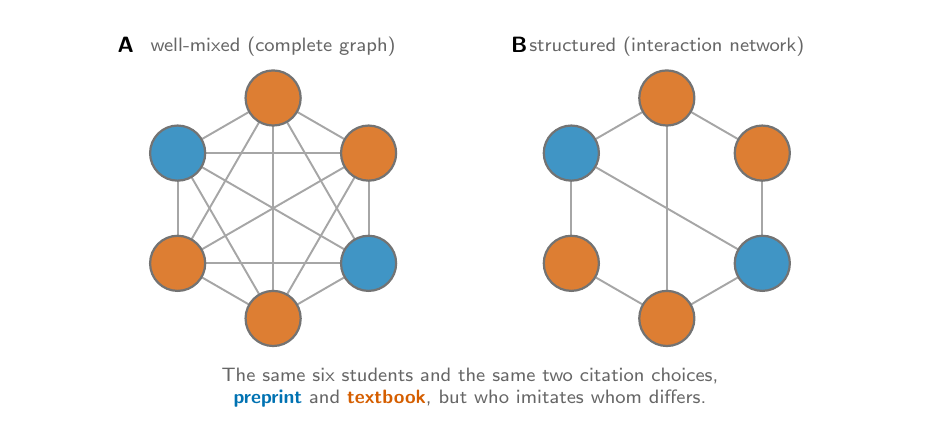
\begin{tikzpicture}[
    font=\sffamily,
    vert/.style={circle, draw=black!55, line width=0.8pt, minimum size=7mm,
                 inner sep=0pt},
    pre/.style={vert, fill=preprint!75, text=white},
    tex/.style={vert, fill=textbook!80, text=white},
    edge/.style={black!35, line width=0.7pt},
    lab/.style={font=\sffamily\scriptsize, text=black!60, align=center},
    panel/.style={font=\sffamily\footnotesize\bfseries, anchor=north west},
]
% colours assigned to the six students (same composition in both panels)
\def\types{{"tex","pre","tex","tex","pre","tex"}}

% ---- Panel A: well-mixed (complete graph) ----
\begin{scope}[shift={(0,0)}]
    \node[panel] at (-2.1,2.3) {A};
    \node[lab] at (0,2.05) {well-mixed (complete graph)};
    \foreach \i in {0,...,5} {
        \coordinate (A\i) at ({90+60*\i}:1.4);
    }
    \foreach \i in {0,...,5} {
        \foreach \j in {0,...,5} {
            \ifnum\i<\j \draw[edge] (A\i) -- (A\j); \fi
        }
    }
    \foreach \i in {0,...,5} {
        \pgfmathparse{\types[\i]}\edef\t{\pgfmathresult}
        \node[\t] at (A\i) {};
    }
\end{scope}

% ---- Panel B: structured (sparse graph) ----
\begin{scope}[shift={(5,0)}]
    \node[panel] at (-2.1,2.3) {B};
    \node[lab] at (0,2.05) {structured (interaction network)};
    \foreach \i in {0,...,5} {
        \coordinate (B\i) at ({90+60*\i}:1.4);
    }
    % a ring with two chords
    \foreach \i [evaluate=\i as \n using {int(mod(\i+1,6))}] in {0,...,5} {
        \draw[edge] (B\i) -- (B\n);
    }
    \draw[edge] (B0) -- (B3);
    \draw[edge] (B1) -- (B4);
    \foreach \i in {0,...,5} {
        \pgfmathparse{\types[\i]}\edef\t{\pgfmathresult}
        \node[\t] at (B\i) {};
    }
\end{scope}

\node[lab, anchor=north, text width=11cm] at (2.5,-1.9)
    {The same six students and the same two citation choices,
     \textcolor{preprint}{\textbf{preprint}} and
     \textcolor{textbook}{\textbf{textbook}}, but who imitates whom differs.};
\end{tikzpicture}
\end{document}
